


\documentclass[8pt,usepdftitle=false]{beamer}
% \imput{../common/beamerthemesimple}
\usetheme{simple}


  \usepackage{xcolor}
  \definecolor{olive}{rgb}{0.3, 0.4, .1}
  \setbeamercolor{itemize/enumerate body}{fg=black}
  \setbeamercolor{title}{fg = green!30!black}
  \setbeamercolor{frametitle}{fg = gray!70!black, bg = white}


% \usepackage{lmodern}
\usepackage[scale = 2]{ccicons}
\usepackage[export]{adjustbox}
\usepackage{amsmath, amsthm, amssymb}
\usepackage{amsfonts}
\usepackage{mathtools}

\usepackage[justification=raggedright,width=\linewidth]{caption}
\usepackage{tikz} 


\usepackage{setspace}

\setbeamertemplate{title page}[default][right,colsep=-4bp,rounded=true,shadow=\beamer@themerounded@shadow]

\setbeamertemplate{caption}[numbered]


%% Options

\setbeamercolor{alerted text}{fg=blue}
\setbeamertemplate{alerted text begin}{\itshape}
\setbeamertemplate{alerted text end}{}

\newenvironment<>{varblock}[2][\textwidth]{%
    \setlength{\textwidth}{#1}
    \begin{actionenv}#3%
        \def\insertblocktitle{\underline{#2}}%
        \par%
        \usebeamertemplate{block begin}}
        {\par%
        \usebeamertemplate{block end}%
    \end{actionenv}}

\setbeamertemplate{blocks}[rounded][shadow=true]
\setbeamercolor{block title}{fg=black,bg=gray!20!white}
\setbeamercolor{block body}{fg=black,bg=gray!10!white}




%% Theorem

% \newtheorem{theorem}{Theorem}

%% Bangla tex


\usepackage{polyglossia}
\setotherlanguage[numerals=Devanagari]{bengali}
\setmainlanguage{english}
\newfontfamily\bengalifont[Script=Bengali]{Akaash}


%% tikx

\usepackage{tikz}
\usetikzlibrary{calc,trees,positioning,arrows,fit,shapes,calc}





\newcommand\blfootnote[1]{%
  \begingroup
  \renewcommand\thefootnote{}\footnote{#1}%
  \addtocounter{footnote}{-1}%
  \endgroup
}



\newcommand\Permute[2][^n]{\prescript{#1\mkern-2.5mu}{}P_{#2}}
\newcommand\Combine[2][^n]{\prescript{#1\mkern-0.5mu}{}C_{#2}}


\renewcommand*{\thefootnote}{\fnsymbol{footnote}}


\usepackage{flexisym}
\usepackage{breqn}

\usepackage[T1]{fontenc}

% \usepackage{mathpazo}
% \renewcommand{\rmdefault}{put}

% \usepackage{fourier} 
% Only use the math font of mathpazo
% \let\temp\rmdefault
% \usepackage{mathpazo}
% \let\rmdefault\temp
% \renewcommand{\rmdefault}{put}


% \usepackage[hyphens]{url}


  % \usefonttheme{professionalfonts} % using non standard fonts for beamer
  % \usefonttheme{serif} % default family is serif

  % \usepackage{gentium}
  \usepackage{multicol}
  \usepackage{mathpazo}



% \renewcommand{\familydefault}{\sfdefault}  


  % color brackets
  \makeatletter
  \newcount\bracketnum
  \newcommand\makecolorlist[1]{%
      \bracketnum0\relax
      \makecolorlist@#1,.%
      \bracketnum0\relax
  }
  \def\makecolorlist@#1,{%
      \advance\bracketnum1\relax
      \expandafter\def\csname bracketcolor\the\bracketnum\endcsname{\color{#1}}%
      \@ifnextchar.{\@gobble}{\makecolorlist@}%
  }
  \let\oldleft\left
  \let\oldright\right
  \def\left#1{%
      \global\advance\bracketnum1\relax 
      \colorlet{temp}{.}%
      \csname bracketcolor\the\bracketnum\endcsname
      \oldleft#1%
      \color{temp}%
  }
  \def\right#1{%
      \colorlet{temp}{.}%
      \csname bracketcolor\the\bracketnum\endcsname
      \oldright#1%
      \global\advance\bracketnum-1\relax
      \color{temp}%
  }
  \makeatother


  \makecolorlist{black,blue,red}






\setbeamertemplate{section in toc}{%
  {\color{firstcolor}\inserttocsectionnumber.}~\inserttocsection}
\setbeamercolor{subsection in toc}{bg=white,fg=black}
\setbeamertemplate{subsection in toc}{%
  \hspace{1.2em}{\color{firstcolor}\rule[0.3ex]{3pt}{3pt}}~\inserttocsubsection\par}


\setbeamerfont{section in toc}{size=\fontsize{6}{8}\selectfont}
\setbeamerfont{subsection in toc}{size=\fontsize{6}{8}\selectfont}
\setbeamerfont{subsection in toc shaded}{size=\fontsize{6}{8}\selectfont}


\makeatletter
\patchcmd{\beamer@sectionintoc}{\vskip1.5em}{\vskip0.5em}{}{}
\makeatother






  \usepackage{twemojis}
  \usepackage{fontspec}
  \usepackage{tikzsymbols}
  \newfontfamily\DejaSans{DejaVu Sans}

% for R
\usepackage[fixed]{fontawesome5}


\setbeamercolor{emph}{fg=red}
\renewcommand<>{\emph}[1]{%
  {\color{purple}\only#2{\rm\itshape}#1}%
}

\setbeamertemplate{frametitle continuation}{}


\usepackage[round,  maxcitenames=10, mincitenames=11]{natbib}
\setlength{\bibhang}{0pt}
\renewcommand{\bibsection}{}
\usepackage{fancybox}


\setbeamertemplate{section page}
{
    \begingroup
    \begin{beamercolorbox}[sep=12pt,center]{section title}
        \usebeamerfont{section title}\insertsection\par
    \end{beamercolorbox}
    \endgroup
}

\setbeamertemplate{subsection page}
{
    \begingroup
    \begin{beamercolorbox}[sep=12pt,center]{section title}
        \usebeamerfont{section title}\insertsection\par
    \end{beamercolorbox}
    \vspace*{-1pt}
    \begin{beamercolorbox}[sep=8pt,center]{subsection title}
        \usebeamerfont{subsection title}\insertsubsection\par
    \end{beamercolorbox}
    \endgroup
}



\newcommand\Var[1]{\mathbb{V}\mathrm{ar}{#1}}



\renewcommand{\emph}[1]{%
{\rm\itshape{\color{purple}#1}}%
}

\renewcommand{\alert}[1]{%
{\rm\itshape{\color{blue}#1}}%
}

\usepackage{hyperref}
\hypersetup{
pdftitle={Chapter 0 - Math Recap - 1},
  pdfsubject={},
  pdfkeywords= {Statistics},
pdfauthor={Hossain},
  pdfborder={0 0 0},
colorlinks,
citecolor=blue,
linkcolor=green!40!black,
breaklinks=true}

\usepackage{cleveref}



\newcounter{mytheorem}
\renewcommand{\themytheorem}{2A.\arabic{mytheorem}}
\newcommand{\Thm}[1]{\refstepcounter{mytheorem}\textbf{#1\color{blue}\themytheorem}:}




%================ Give the title ============================##

\title{\LARGE Ch0 - Math Recap - 1}

\subtitle{{\fontsize{10}{10}\selectfont\color{gray!50!balck} 
(\rm \itshape Sets and Related Ideas)}
\\\vspace*{.2cm} \scshape ECO 104 - Statistics For Business and Economics - I}

\author{Shaikh Tanvir Hossain\vspace*{-.4cm}}
\institute{ East West University, Dhaka\\  \today}
\date{\vspace{-5pt}}
% \titlegraphic{\includegraphics[width=300,height=.5\textheight]{Images/EWU.png}}

% \setbeamertemplate{background}{\tikz[overlay,remember picture]\node[opacity=0.90]at (current page){\includegraphics[width=.5\textwidth,left]{EWU.png}};}


\begin{document}



\begin{frame}[plain,noframenumbering] 
    \maketitle
\end{frame}
\setbeamertemplate{background}{}
\setlength{\abovedisplayskip}{-2pt}
\setlength{\belowdisplayskip}{4pt}
\setlength{\abovedisplayshortskip}{-3pt}
\setlength{\belowdisplayshortskip}{4pt}


\AtBeginSection[]
{
    \begin{frame}[plain, allowframebreaks]
\setstretch{.1}

        \setlength{\parskip}{1ex}
            \tableofcontents[sections={1-7}, 
            currentsubsection, 
            sectionstyle=show/hide, 
            sectionstyle=show/shaded, 
            ]
    \end{frame}
}


% Hide progress bar and footline on titlepage
\begin{frame}{Outline}
 \vspace*{.2cm}

\begin{center}
\begin{minipage}{10cm}
  \begin{alertblock}{Outline}
  \setstretch{.1}
   \setlength{\parskip}{1ex}
  \tableofcontents[sections={1-10}]
  %   \framebreak
  % \tableofcontents[sections={2}]
\end{alertblock}
\end{minipage}
\end{center}


\end{frame}




%---------------------------------------------------------------------------------
%---------------------------------------------------------------------------------
%---------------------------------------------------------------------------------


\begin{frame}[allowframebreaks]{Regarding Math Recap}
  
\textbf{We need some Math!}

\begin{enumerate}
\item We will need some math in this course, so first we will do a quick recap!
\item This is going to be Math Recap Part 1, where we will cover mainly \alert{sets}
\item In Part 2 Recap we will we will cover \alert{functions, and some counting methods!}, but that will come before Probability theory in Chapter 2.
\end{enumerate}

\textbf{But don't worry!}
\begin{enumerate}
\item These math topics should be familiar to you.
\item Most of you have already studied College-Level math (H.S.C Math or A Level Math) or at least took Math 100 at EWU.
\end{enumerate}

\textbf{But still....}
\begin{enumerate}
\item If you feel a bit rusty with these concepts, please take the time to go through the material.
\item Note that this recap is not a replacement for a full math course but is intended to refresh your knowledge on essential topics.
\item So let's start with the recap!
\end{enumerate}
\end{frame}


\section{Sets}
\subsection{a. Definitions and Examples}
\frame{\subsectionpage}
%---------------------------------------------------------------------------------


\begin{frame}[allowframebreaks]{Sets and Related Ideas}{Basic Definitions}

\begin{itemize}

      \begin{block}{\Thm{Definition~}(Set) }
           A set is a \emph{collection of objects} treated as a \emph{single} entity, the members are called \emph{elements}.  If $X$ is a set and $x$ is an element, we write $x \in X$, and this reads as "$x$ belongs to $X$".
        \end{block}
        \medskip


\item Note the symbol $\in$ means ``belongs to''. For example, think about the set of even numbers between $1$ and $11$, if we \emph{enumerate} then we can write this set as $  S=\{2,4,6,8,10\}$. Note in this case, $2, 4, 6, 8, 10$ are all elements of the same set, so we can write $2 \in S$, $4 \in S$, and so on...

\medskip

\item Now in math we can write the same set also as,  

\begin{align*}
S=\{x: x \text{ is an even number between } 1 \text{ and } 11\}
\end{align*}

\item Where this means \emph{``$S$ is a set of element $x$, such that $x$ is an even number between $1$ and $11$''}, note the symbol ":" means \alert{"such that"}. 


\framebreak

\item Note we wrote the same set in two different ways, 

\item The first method is called \emph{enumeration method} 

\item And the second one is called \emph{set builder method}. 

\item Sometimes you will also see a slightly different notation ``$\mid$'' instead of ``$:$''. For example, we can write the same set as  

\begin{align*}
S=\{x \mid x \text{ is an even number between } 1 \text{ and } 11\}
\end{align*}

\item Question: What's the benefit of set builder method?


\framebreak

\item Now we will see some quick definitions related to set.

\item \textbf{\emph{Empty Set:}} When a set has no element, then we call this an \alert{empty set}. This set is denoted by $\emptyset$ or $\{\}$.

\item \textbf{\emph{Equal Sets:}} Two sets $X$ and $Y$ are equal if they contain exactly the same elements. and we write $X=Y$

\item \textbf{\emph{Subset:}}   If we have two sets $X$ and $Y$, and all the elements of a set $X$ are also elements of the set $Y$, then $X$ is a called a \alert{subset} of $Y$, and we use the notation $X \subset Y$. Note that in this case $Y$ is also called a \alert{superset} of $X$. 


\item \textbf{\emph{Proper Subset:}} Note when we write $X \subset Y$, then the set $X$ may have exactly same elements as $Y$ or may have less than $Y$. If all the elements in set $X$ are in a set $Y$, but not all the elements of $Y$ are in $X$, then $X$ is called a \alert{proper subset} of $Y$. In this case $X$ must have less number of elements. The notation is $X \subsetneq Y$. 

\framebreak

\item \emph{An Interesting Point: Note that empty set $\{ \}$ is a subset of any set, why?} 

\item Ans: This is because even if we think what belongs to empty set also belongs to another set, this is always true, since empty set contains nothing. We sometimes call this \emph{Vacuously True}!

\begin{figure}[H]

\includegraphics[scale = .5]{Images/nothing.png}
\end{figure}


\item Let's do some examples 
\medskip

\Thm{Example \label{E1.1}}~Suppose we have following sets,
\medskip


\begin{align*}
A = \{a, b, c \}, \quad B = \{a, b, c \}, \quad C = \{b, c\} \text{ and } D = \{c\}
\end{align*}



 \item[] Then we can see that $A = B$, but $A \neq C$ and also $B \neq C$ and also $C \neq D$. 

\item[] Also note $A \subset B$, and also $B \subset A$,  $C \subset B$ and also $D \subset C$, and also $C \subsetneq B$ (\alert{Question:} Is it correct to write $D \in C$, Ans: No, why?)

\end{itemize}
\end{frame}


\subsection{b. Set Operations}
\frame{\subsectionpage}
\begin{frame}[allowframebreaks]{Sets and Related Ideas}{Set Operations}

\begin{itemize}



\item Now we will see some concepts which we call \emph{Set Operations}. Set operations mean we will combine two or more sets in different ways. Following are important set operations.
    
\item \textbf{1. Union of two sets:} The union of two sets $A$ and $B$ is the set of elements that belong \emph{either} set $A$ \emph{or} set $B$ or \emph{both} of the sets. The notation we will use is $A \cup B$. So this means




\begin{align*}
A \cup B=\{ x: x \in A \text { OR } x \in B\}
\end{align*}


\item \textbf{2. Intersection of two sets:} The intersection of two sets $A$ and $B$ is the set of elements that belong to \alert{both} $A$ and $B$. We will use the notation $A \cap B$. So


\begin{align*}
A \cap B=\{x: x \in A \text { AND } x \in B\}
\end{align*}


\item \textbf{3. Difference between two sets:} The difference (sometimes also called relative difference) of $A$ and $B$ is the set of elements that \alert{belong to} $A$ but \alert{not belong to} $B$. The notation is $A \setminus B$. We can write,



\begin{align*}
A \setminus B=\{x: x \in A \text { and } x \notin B\}
\end{align*}



\item \textbf{4. Product of two sets:} If $A$ and $B$ are sets, then the product of two sets is called \emph{Cartesian product}. The \alert{Cartesian product} of $A$ and $B$ is the \emph{set} of all \alert{ordered pairs} $(a, b)$ such that $a \in A$ and $b \in B$. So using set building notation we can write,


\begin{align*}
A \times B=\{(a, b): a \in A \text { and } b \in B\}
\end{align*}

\item Note in the Cartesian Product \emph{ordering} is important. For two sets $A$ and $B$, $A \times B$ is not same as $B \times A$ (look at the next example).




\framebreak

\Thm{Example \label{E1.7}}~Suppose we have following sets,

\begin{align*}
A = \{a, b, c \}, \quad B &= \{a, b, c \}, \quad C = \{b, c\}, \\
D = \{c\}, \quad & E = \{1, 2\}
\end{align*}

Now $A \cup B = \{a, b, c \}$, $C \cup D = \{b, c\}$, $C \cap D = \{c\}$, $B \setminus C = \{ a\}$. 

\medskip
Let's think about Cartesian Products,

\begin{align*}
A \times E = \{a, b, c \} \times \{1, 2\} =  \{(a, 1), (a, 2), (b, 1), (b, 2), (c, 1), (c, 2) \} \text{ but } \\
E \times A =  \{ 1, 2 \} \times \{ a, b, c \} =  \{ (1, a), (1, b), (1, c), (2, a), (2, b), (2, c) \} 
\end{align*}




\item Note that, \alert{ordering matters} for the product of sets, so $(a, 1) \neq (1, a)$. So $ A \times E \neq E \times A$.

\framebreak

\textbf{Idea of the Universal Set and Complements}\\



\item Often (depending upon the problem) we have a \emph{universal set}. The idea of the universal set is, it acts like a ``\emph{Universe}'', this means everything belongs here. We usually denote the universal set with $U$ (see example below)

\begin{align*}
U = \{a, b, c, 1, 2\}, \\
\quad A = \{a, b, c \}, \quad B = \{a, b, c \}, \quad C = \{b, c\}\quad&  D = \{c\}, \quad E = \{1, 2\} \\
\text{ Note that all sets are subsets of the Universal Set } U
\end{align*}

\item Now once we have a universal set, then we can find a complement of which is the remaining part of the Universal set. For example, take the set $A$ from the last example, here $A \subset U$, then the complement set is 

\begin{align}
    A^{c} = U \setminus A
\end{align}

for complement sometimes there is another notation $\bar{A}$, I think \citet*{chiang_2005} uses this notation.



\item \Question{What is $B^{c}$ and $C^{c}$?}

\framebreak

\item We can have a visual understanding of union, intersection, complement and set difference using a diagram called \emph{Venn diagram}. 

\item What is a Venn Diagram? The idea of the Venn diagram is to show these concepts visually with balls and squares (A famous mathematician, logician and philosopher Jonn Venn (1834 – 1923) came up with this idea!)

\item Here are some Venn Diagrams for the concepts we have learned so far. 



\begin{figure}[H]
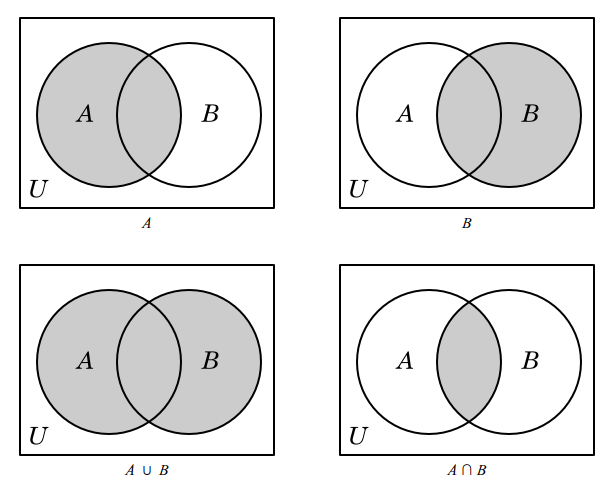
\includegraphics[scale = .3]{Images/Venndiagrams_part1.png}
\caption{Venn diagram for $A\cup B$, $A\cap B$ }
\end{figure}




\begin{figure}[H]
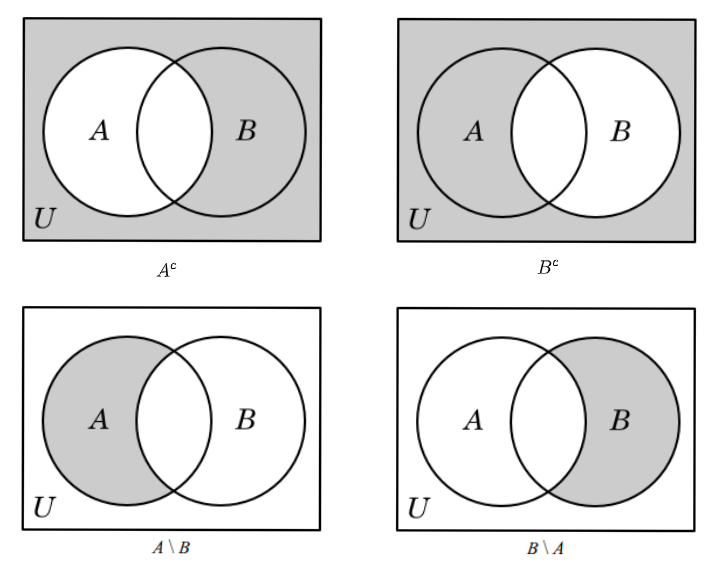
\includegraphics[scale = .25]{Images/Venndiagrams_part2.png}
\caption{Venn diagram for $A^{c}$, $B^{c}$, $A \setminus B$, \text{ and } $B \setminus A$ }
\end{figure}





\framebreak

\item The idea of Unions, Intersections, Cartesian Product and also Difference can be easily extended to more than two sets. In this case the idea is same, you just apply this similarly (this is the beauty of Math!)


\item For example if we have a \alert{sequence of sets} $A_1, A_2, A_3$, then for union and intersection we will have,

\begin{align*}
A_1 \cup A_2 \cup A_3 \text{ and } A_1 \cap A_2 \cap A_3
\end{align*}

\item For Cartesian Product we can also do 

\begin{align*}
A_1 \times A_2 \times A_3
\end{align*}

\item And for difference we also have 

\begin{align*}
A_1 \setminus A_2 \setminus A_3
\end{align*}


\item Think about some examples?


\framebreak

\item Now we will learn some \emph{laws / rules for sets when it comes to combining the operations like unions, intersections and difference}.

\item I will just mention three laws, which are the most fundamental ones, but it is possible to construct more. Laws means these are some mathematical statements that we need to prove (careful : this is not definition, for definition / axioms there is no proof, we just take them as it is). In general in Math we need to prove statements which are laws / rules / theorems / corollary / propositions / lemma ... but we will not do any proof here, maybe in higher courses you will learn some how to do mathematical proof, here we will simply learn the rules and apply them!




\begin{block}{Laws of Sets (Associative, Distributive and De-Morgan's Law)}
    
\begin{itemize}
\item \emph{Associative Law} 

\begin{align*}
\text{1. } A \cup (B \cup C) &= (A \cup B)\cup C\\
\text{2. } A \cap (B \cap C) &= (A \cap B)\cap C
\end{align*}


\item  \emph{Distributive Law} 


\begin{align*}
\text{1. } A \cup (B \cap C) &= (A \cup B)\cap (A \cup C) \\
\text{2. } A \cap (B \cup C) &= (A \cap B) \cup (A \cap C)
\end{align*} 

\item \emph{Demorgan's Law}

\begin{align*}
\text{1. } (A \cap B)^c &= A^{c} \cup B^{c} \\
\text{2. } (A \cup B)^c &=  A^{c} \cap B^{c} 
\end{align*}

\end{itemize}

\end{block}



\item Although we won't do any proof here, but it's very important that we understand the laws properly.

\item The first law says - if we first take the union of the sets $B$ and $C$ and then take the union of $A$ with the result of $B \cup C$, then this will be same as first taking the union of $A$ and $B$ and then taking the union of $A \cup B$ with $C$. 


\item Can you interpret others?


\item Let's do an example, Let's verify the first distributive law, Let $A=\{4,5\}, B=\{3,6,7\}$, and $C=\{2,3\}$. 

\item To verify the first part of the law, we find the left- and right-hand expressions separately:

\item \emph{Calculation for Left:} first calculate $B \cap C = \{ 3 \}$ and then $A \cup (B \cap C)$, we get $A \cup(B \cap C)=\{4,5\} \cup\{3\}=\{3,4,5\}$

\item \emph{Calculation for the right:} first calculate $A \cup B = \{3,4,5,6,7\}$ and then $A \cup C = \{2,3,4,5\}$, now we do $(A \cup B) \cap (A \cup C)$ and here  $(A \cup B) \cap (A \cup C) = \{3,4,5\}$


\framebreak

\textbf{Power Set : The set of all possible subsets}\\

\item Now let's talk about the \alert{Power Set}. Power set is actually \alert{a set of sets}


\item The power set of a set $A$, is a \alert{set of of all possible subsets of $A$}. The notation for power set of $A$ is $\mathcal{P}(A)$.

\vspace*{.3cm}

\Thm{\small Example } (Power Set)

\begin{itemize}
  \item If we have a set $A = \{1, 2\}$, then $\mathcal{P}(A) = \Big\{  \{\}, \{1\}, \{2\}, \{1, 2\} \Big\}$.
  \item If we have a set $A = \{1, 2, 4\}$, then 

  \begin{align*}
    \mathcal{P}(A) &= \Big\{ \{\}, \{1\}, \{2\}, \{1, 2\}, \{4\}, \{1, 4\}, \{2, 4\}, \{1, 2, 4\} \Big\} \\
    &= \Big\{ \emptyset, \{1\}, \{2\}, \{1, 2\}, \{4\}, \{1, 4\}, \{2, 4\}, A\Big\}
  \end{align*}

  \item If we have a set  $B = \{a, b, c, d\}$, calculate $\mathcal{P}(B)$

  \item If we have a set $\Omega = \{H, T\}$, calculate $\mathcal{P}(\Omega)$

   \item If we have a set $\Omega = \{1, 2, 3, 4, 5, 6\}$, calculate $\mathcal{P}(\Omega)$
\end{itemize}


\item So in simple words, a \alert{power set is a set of sets} which has all the subsets that we can construct with the elements of $A$.

\item Often a \alert{set of sets} is called a \alert{family of sets}.


  \item There is a nice trick which we can use to count the number of elements in the power set if the given set is countable and finite. For example if $A$ is a \alert{countable and finite set}\footnote[frame]{Question is what does countable mean in Mathematics? It means - we can \alert{enumerate} the elements. A set can be countably finite, countably infinite and uncountable. Uncountable sets are always infinite, it is not possible to have uncountable but finite sets. Examples.....(on board)} then $\mathcal{P}(A)$ will have $    2^{(\text{number of elements in } A)}$








\item For example, if $A = \{1, 2\}$, then the power set $\mathcal{P}(A)$ will have $2^2 = 4$ elements. Note that this matches with our earlier answer. 


\item Can you think about power set of $\mathbb{R}$, so this means can you think about $\mathcal{P}(\mathbb{R})$? (This is huge right but maybe an idea?)



\end{itemize}


\end{frame}


\subsection{c. Different Sets of Numbers}
\frame{\subsectionpage}
\begin{frame}[allowframebreaks]{Sets and Related Ideas}{Sets of Numbers}




\begin{itemize}
\item There are different \alert{sets of numbers} in mathematics. 
\vspace*{.1cm}


\begin{itemize}
\item \alert{Set of Real numbers}, we use the notation $\mathbb{R}$ to denote this set. This set include all numbers that you can possibly think about (except complex numbers, which we don't need now). This is a huge set which is \alert{uncountable} and of course \alert{infinite}.

\medskip

\item \alert{Set of Natural numbers}, we use the notation $\mathbb{N}$. This set include all positive integer numbers $1, 2, 3, 4, \ldots, $. This is a \alert{countable set} but an infinite set, so this is a \alert{countably infinite} set (are you wondering what does countable mean?).

\medskip

\item \alert{Set of Integer numbers}, we use the notation $\mathbb{Z}$. This set include all the positive and negative integer numbers $\ldots, -3, -2, -1, 0, 1, 2, 3, \ldots$. This is also a \alert{countably infinite set}. Note that $\mathbb{N} \subsetneq \mathbb{Z} $

\medskip

\item \alert{Set of Rational numbers}, we use the notation $\mathbb{Q}$. This set include the numbers which can be written as fractions $p/q$, where $p$ and $q$ are both integers. This set has numbers like $2/3, 10/3$ and also all positive and negative integers are also part of this set (why?). This is also a \alert{countably infinite set}.  $\mathbb{N} \subsetneq \mathbb{Z} \subsetneq \mathbb{Q} $

\medskip

\item \alert{Set of Irrational numbers}. Everything that is NOT Rational but in $\mathbb{R}$ is part of this set, for example $\sqrt{2}$, We can write this set with $\mathbb{R} \setminus \mathbb{Q}$.

\medskip

\item This means we can write $\mathbb{N} \subsetneq \mathbb{Z} \subsetneq \mathbb{Q} \subsetneq \mathbb{R}$



\end{itemize} 




\item The set of real numbers $\mathbb{R}$ can be also visualized in the numberline, here is the numberline that you are probably familiar with

\vspace*{.3cm}
\begin{figure}
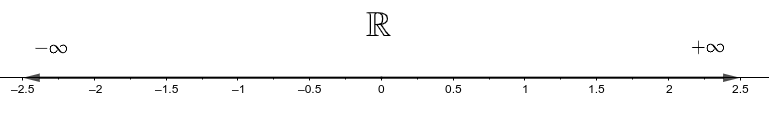
\includegraphics[scale = .5]{Images/x_axis.png}
\end{figure}

\item At the center, we have the number $0$ (this is often called the origin or center), at left the number goes to $-\infty$ and right it goes to $\infty$.

\item We can point any number that belongs to $\mathbb{R}$ in the numberline. Here we showed only a few.






\item We can also have different kinds of intervals in $\mathbb{R}$, which are also subsets of $\mathbb{R}$. For example we can construct following intervals (here $a$ and $b$ can be any number in $\mathbb{R}$)
\vspace*{.2cm}


\begin{figure}
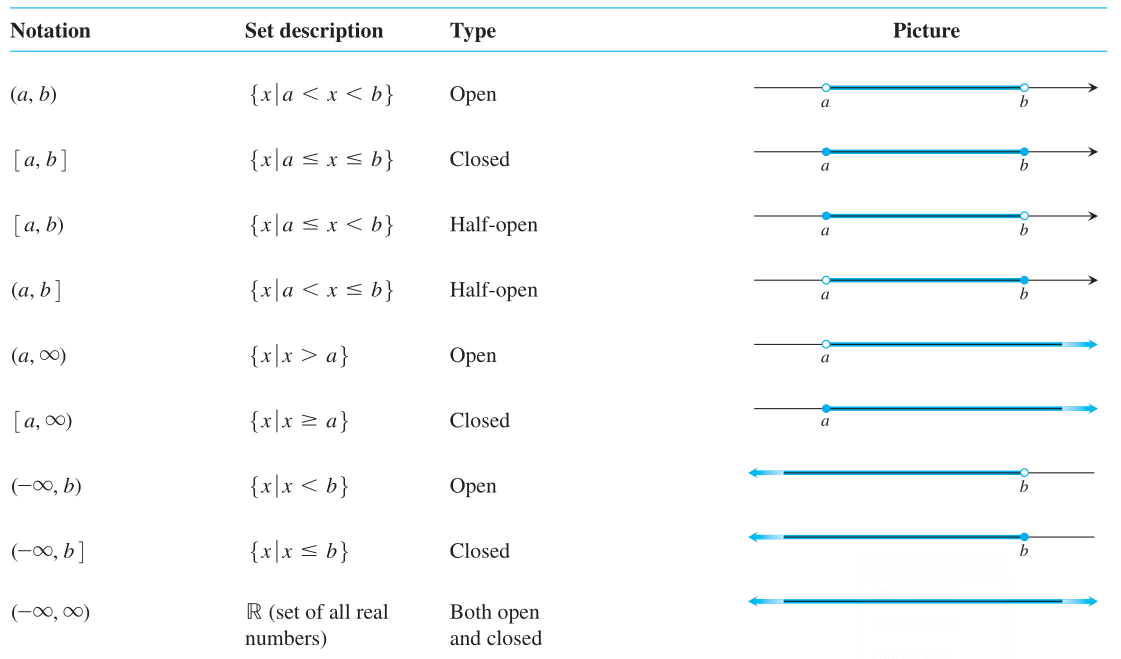
\includegraphics[scale = .28]{Images/Intervals2.png}
\end{figure}

\item Intervals like $(a, b)$  is called \alert{open intervals}, intervals like $[a, b]$ \alert{closed intervals}, intervals like $(a, b]$ or $[a, b)$ are called \alert{half-open} intervals.



\item Recall the idea of Cartesian product? Can you think about the Cartesian product $\mathbb{R} \times \mathbb{R}$? Although it is impossible to write the set $\mathbb{R} \times \mathbb{R}$, but we can visualize it. 

\item Just put another numberline vertically on top of the horizontal one, then we will have something which is known as \alert{Cartesian Coordinate} or \alert{$x-y$ Coordinate} or \alert{$x-y$ plane}

\item Now here we have a horizontal axis, known as $x$-axis, and the vertical axis, known as $y$-axis.




\begin{figure}
\centering
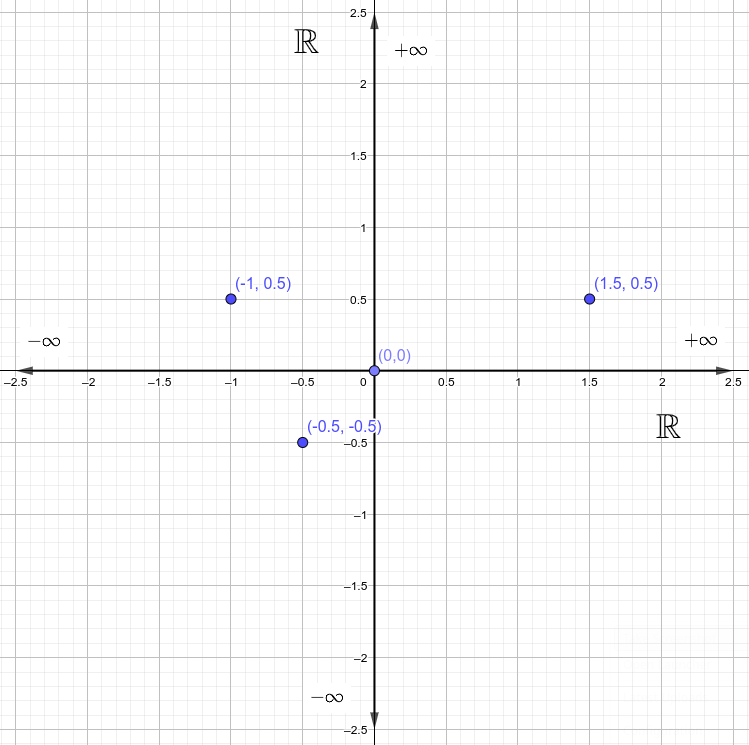
\includegraphics[scale = .25]{Images/cartesian_coordinate.png}
\end{figure}




\begin{itemize}


\item Here we can show any pair of numbers $(x, y)$, where the first number is on the $x$-axis and the second is on the $y$-axis, and togther we can locate the point $(x, y)$ on this $x-y$ plane.


\item We have showed the center, which is at $(0, 0)$, and also other three points,  $(-1, 0.5)$, $(1.5, 0.5)$ and $(-0.5, -0.5)$

\end{itemize}



\begin{figure}
\centering
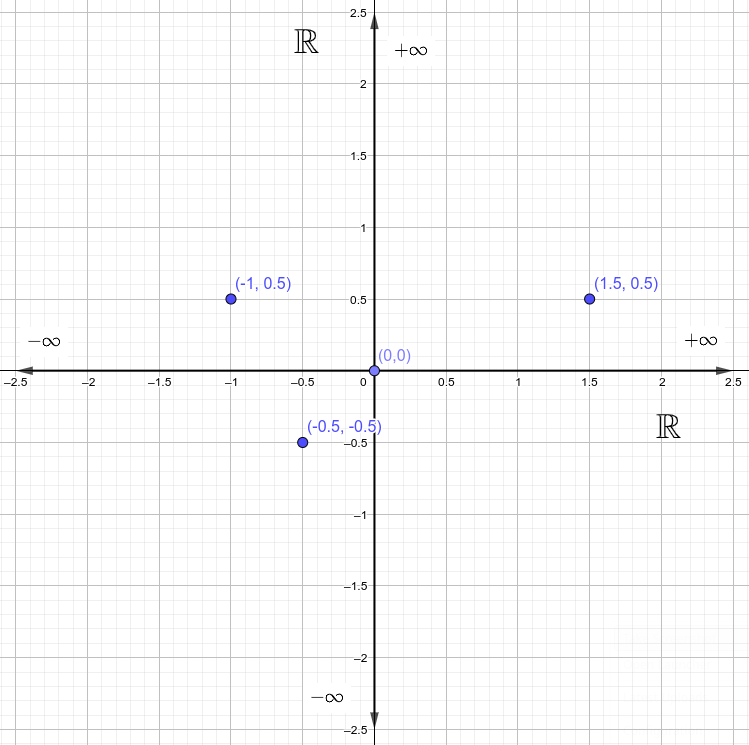
\includegraphics[scale = .25]{Images/cartesian_coordinate.png}
\end{figure}




\end{itemize}
\end{frame}





\section{Functions and Related Ideas}
\frame{\sectionpage}


\begin{frame}[allowframebreaks]{Functions and Related Ideas}

\begin{itemize}
\item If you have taken any math courses, whether in college or courses like MAT100 or MAT110, you have definitely seen functions. 

\item For example following are all examples of functions,

\begin{itemize}
\item $f(x) = x^2$
\item $f(x) = 2x + 1$
\item $f(x) = 3x^3 + 2x^2 + 1$
\end{itemize}

\item It is very easy to understand a function, there is always \emph{an input} and and \emph{an output}, and the function specifies this input-output relation. Important is for each input there is only one output, there cannot be more than one.


\item Following picture might be helpful


\begin{figure}
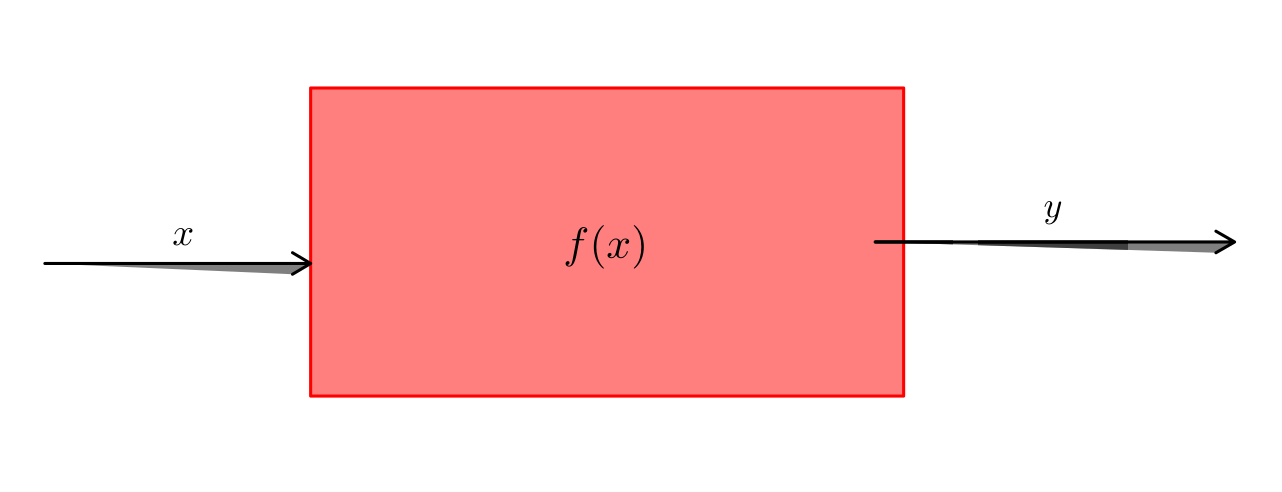
\includegraphics[scale = .2]{Images/function_1.png}
\caption{A function, we write $y = f(x)$ specifies a process here $x$ can be viewed as an input and $y$ or $f(x)$ is the output.}
\end{figure}

\framebreak



\item Formal definition of definition is similar, it just makes the definition more precise.

\begin{block}{\Thm{Definition \label{d1.}} (Function) }
Given any two sets $A$ and $B$, a function $f: A \to B$ is a \alert{mapping} between the elements of $A$ and $B$ such that the following condition is satisfied 

\begin{itemize}
\item For every element of $A$ there is a unique element in $B$.
\end{itemize}    

In this case, the set $A$ is called the \alert{domain} of the function $f$ and $B$ is called the \alert{codomian} of the function.

\end{block}



\item It is important to mention that although in the definition we wrote one condition, that is \alert{"For every element of $A$ there is a unique element in $B$."}, this actually means two points,

\begin{itemize}
\item  First, Since we are saying "For \alert{every} element of $A$...", the word ``every'' here automatically means all elements of  $A$ needs to be used for mapping .

\item[]

\item Second, when we say for each element of $A$, there must be a unique element in $B$. This means it will never happen that a single point from $A$ is mapped to two different points in $B$.
\end{itemize}

\item We won't go to more details here, please MAT-100 / College Math notes if you need to brush up!


\end{itemize}



\end{frame}



% \item Let's see some examples, suppose we have two sets $A = \{p, q, r, s \}$ and $B = \{1, 2, 3, 4, 5\}$. Here the domain is $A$ and the codomain is $B$. Question - Is the following mapping a function? Answer - Yes it is, how? 

% \begin{figure}\label{fig:functions1}
% \centering
% \begin{tikzpicture}[ele/.style={fill=black,circle,minimum width=.4pt,inner sep=1pt},every fit/.style={ellipse,draw,inner sep=-0.3pt}]
% \node[ele,label=left:$p$] (a1) at (0,3) {};    
% \node[ele,label=left:$q$] (a2) at (0,2.5) {};    
% \node[ele,label=left:$r$] (a3) at (0,2) {};
% \node[ele,label=left:$s$] (a4) at (0,1.5) {};
% \node[ele,label=left:$\,$, color = white] (a5) at (0,1) {};


% \node[ele,,label=right:$1$] (b1) at (4,3) {};
% \node[ele,,label=right:$2$] (b2) at (4,2.5) {};
% \node[ele,,label=right:$3$] (b3) at (4,2) {};
% \node[ele,,label=right:$4$] (b4) at (4,1.5) {};
% \node[ele,,label=right:$5$] (b5) at (4,1) {};

% \node[draw,fit= (a1) (a2) (a3) (a4),minimum width=2cm, minimum height=3.3cm] {} ;
% \node[draw,fit= (b1) (b2) (b3) (b4),minimum width=2cm, minimum height=3.3cm] {} ; 


% \draw[->,thick,shorten <=2pt,shorten >=2pt] (a1) -- (b1);
% \draw[->,thick,shorten <=2pt,shorten >=2] (a2) -- (b2);
% \draw[->,thick,shorten <=2pt,shorten >=2] (a3) -- (b4);
% \draw[->,thick,shorten <=2pt,shorten >=2] (a4) -- (b3);


% \node[label=$A$] () at (0,-.25) {};
% \node[label=$B$] () at (4,-.25) {};
% \end{tikzpicture}
% \vspace*{-.5cm}
% \caption{This is a mapping between two sets $A$ and $B$. In general mapping can be any relation between the two sets. However this mapping is a function (check the condition) and we can call this function $f$, also we can write  $f : A \to B$.}
% \end{figure}

% \framebreak

% \item Following is not a function. It is important to understand that here there is a viloation of the condition. In particular it violates the second point in page 23. So it is {\color{red}NOT a function}.

% \begin{figure}\label{fig:functions1}
% \centering
% \begin{tikzpicture}[ele/.style={fill=black,circle,minimum width=.4pt,inner sep=1pt},every fit/.style={ellipse,draw,inner sep=-0.3pt}]
% \node[ele,label=left:$p$] (a1) at (0,3) {};    
% \node[ele,label=left:$q$] (a2) at (0,2.5) {};    
% \node[ele,label=left:$r$] (a3) at (0,2) {};
% \node[ele,label=left:$s$] (a4) at (0,1.5) {};
% \node[ele,label=left:$\,$, color = white] (a5) at (0,1) {};


% \node[ele,,label=right:$1$] (b1) at (4,3) {};
% \node[ele,,label=right:$2$] (b2) at (4,2.5) {};
% \node[ele,,label=right:$3$] (b3) at (4,2) {};
% \node[ele,,label=right:$4$] (b4) at (4,1.5) {};
% \node[ele,,label=right:$5$] (b5) at (4,1) {};

% \node[draw,fit= (a1) (a2) (a3) (a4),minimum width=2cm, minimum height=3.3cm] {} ;
% \node[draw,fit= (b1) (b2) (b3) (b4),minimum width=2cm, minimum height=3.3cm] {} ; 


% \draw[->,thick,shorten <=2pt,shorten >=2pt] (a1) -- (b1);
% \draw[->,thick,shorten <=2pt,shorten >=2] (a1) -- (b2);
% \draw[->,thick,shorten <=2pt,shorten >=2] (a2) -- (b3);
% \draw[->,thick,shorten <=2pt,shorten >=2] (a3) -- (b4);
% \draw[->,thick,shorten <=2pt,shorten >=2] (a4) -- (b5);


% \node[label=$A$] () at (0,-.25) {};
% \node[label=$B$] () at (4,-.25) {};
% \end{tikzpicture}
% \vspace*{-.5cm}
% \caption{Note that this violates the condition, because for the element $p$ we don't have a unique element in $B$, rather we have two elements $1$ and $2$.}
% \end{figure}

% \framebreak

% \item Following {\color{red}is a function}, and there is no problem with the condition.

% \begin{figure}\label{fig:functions1}
% \centering
% \begin{tikzpicture}[ele/.style={fill=black,circle,minimum width=.4pt,inner sep=1pt},every fit/.style={ellipse,draw,inner sep=-0.3pt}]
% \node[ele,label=left:$p$] (a1) at (0,3) {};    
% \node[ele,label=left:$q$] (a2) at (0,2.5) {};    
% \node[ele,label=left:$r$] (a3) at (0,2) {};
% \node[ele,label=left:$s$] (a4) at (0,1.5) {};
% \node[ele,label=left:$\,$, color = white] (a5) at (0,1) {};


% \node[ele,,label=right:$1$] (b1) at (4,3) {};
% \node[ele,,label=right:$2$] (b2) at (4,2.5) {};
% \node[ele,,label=right:$3$] (b3) at (4,2) {};
% \node[ele,,label=right:$4$] (b4) at (4,1.5) {};
% \node[ele,,label=right:$5$] (b5) at (4,1) {};

% \node[draw,fit= (a1) (a2) (a3) (a4),minimum width=2cm, minimum height=3.3cm] {} ;
% \node[draw,fit= (b1) (b2) (b3) (b4),minimum width=2cm, minimum height=3.3cm] {} ; 


% \draw[->,thick,shorten <=2pt,shorten >=2pt] (a1) -- (b1);
% \draw[->,thick,shorten <=2pt,shorten >=2] (a2) -- (b1);
% \draw[->,thick,shorten <=2pt,shorten >=2] (a3) -- (b2);
% \draw[->,thick,shorten <=2pt,shorten >=2] (a4) -- (b3);


% \node[label=$A$] () at (0,-.25) {};
% \node[label=$B$] () at (4,-.25) {};
% \end{tikzpicture}
% \vspace*{-.5cm}
% \caption{Here although both $p$ and $q$ are mapped to the same elements but still it does not violate the condition.}
% \end{figure}

% \item For the notation of functions, usually we use the letters $f$, $g$, $h$, etc. Sometimes when we write many functions we also use index $1, 2, 3, \ldots, $. For example $f_{1}, f_{2}, f_{3}, \ldots,$ and so on.


% \item Always remember when we write $f : X \to Y$, this means $f$ is a function, $X$ is the domain and $Y$ is the codomain. 

% \framebreak

% \item  Using the function notation for the last example we can write 

% \begin{align*}
% f(p) &= 1, \\
% f(q) &= 2, \\
% f(r) &= 4 \text{ and } \\
% f(s) &= 3
% \end{align*}

% \item and we can write $f: A \to B$.

% \item There is another set in function, which is called \alert{range of a function}. Range is simply the subset of the co-domain which is used the in the mapping. So for the last example the set $B = \{1, 2, 3, 4, 5 \}$ is the \alert{codomain} and  $\{1, 2, 3, 4\}$ is the \alert{range}.  


% \item Question  - Note we did not use all the elements in $B$ in Figure 3 to represent a function. Is this a problem with the definition of a function? (Answer is NO, why?)

% \item Question  - For these two sets can you draw some mappings which are not functions? (Try this now, Hint: Just intentionally violate the two points mentioned in page 23.)

% \framebreak

% \item The functions that you already know or have seen, for example, 

% \begin{itemize}
% \item  1. $f(x) = x^2$
% \item 2. $f(x) = 2x + 1$
% \item 3. $f(x) = 3x^3 + 2x^2 + 1$
% \end{itemize} 

% are all examples functions where we used \alert{algebraic expressions}. We write functions in this way when the domain and codomain are infinite or uncountable sets. 


% \item Note that for above three functions, 

% \begin{itemize}
% \item  1. $f(x) : \mathbb{R} \to \mathbb{R}$, domain and codomain - $\mathbb{R}$ and range $\mathbb{R}_{\geq 0}$
% \item 2.  $f(x) : \mathbb{R} \to \mathbb{R}$, domain, codomain and range $\mathbb{R}$
% \item 3.  $f(x) : \mathbb{R} \to \mathbb{R}$, domain, codomain and range $\mathbb{R}$
% \end{itemize}



% \framebreak



% \item Here the functions are mapping between two huge sets, so we cannot draw pictures like Figure 3. But definitely when we have a \alert{graph of the functions} then we can see also see the connections between the domian $\mathbb{R}$ and the co-domain $\mathbb{R}$. 

% \vspace*{.2cm}
% \begin{figure}
% 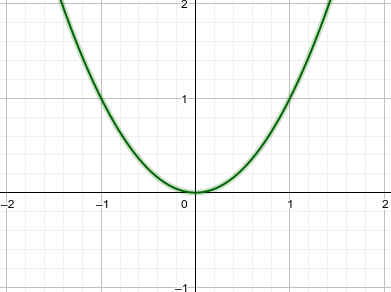
\includegraphics[scale = .3]{Images/fx_1.png}
% 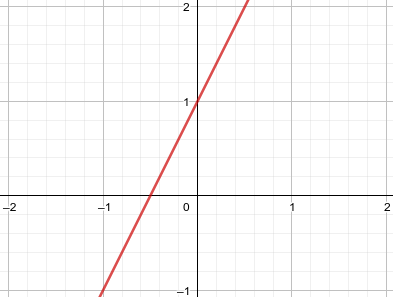
\includegraphics[scale = .3]{Images/fx_2.png}
% 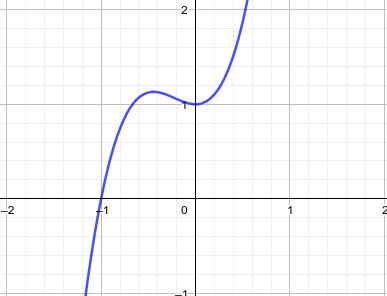
\includegraphics[scale = .3]{Images/fx_3.png}
% \caption{From left - $f(x) = x^2$, $f(x) = 2x + 1$ and $f(x) = 3x^3 + 2x^2 + 1$}
% \end{figure}





% \item Question - If we draw any line on the $x-y$ coordinate, is it always going to be a function?

% \item For example, is the following a function? We can write this equation as $x = y^2$


% \begin{figure}
% 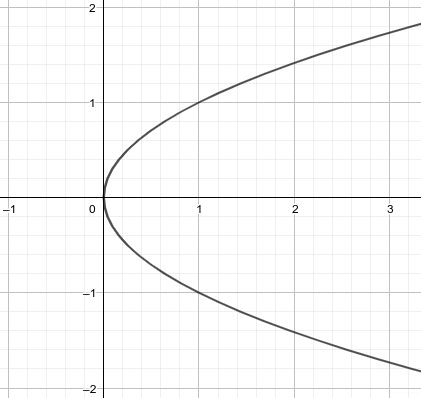
\includegraphics[scale = .4]{Images/fx_4.png}
% \end{figure}

% \item NO! why? Do a vertical line test.

% \framebreak



% \item An important type of functions is called \emph{polynomial function}

% \item A polynomial of degree $n$ is a function of the form

% $$
% f(x)= a_0 + a_1x + a_2 x^2 + \ldots + a_n x^n
% $$

% \item where the $a$ 's are real numbers (sometimes called the coefficients of the polynomial), and $x$ is the input of the function

% \item Although this general formula might look quite complicated, particular examples are much simpler. 

% \item For example,

% $$
% f(x)= 2 + x^2 + 3x^3 
% $$

% is a polynomial of degree 3 , as 3 is the highest power of $x$ in the formula. This is called a \emph{cubic function} 

% \item And

% $$
% f(x)= 1 + x^5 + x^7
% $$

% is a function with polynomial of degree 7 , as 7 is the highest power of $x$. 

% \framebreak 

% \item Notice here that we don't need every power of $x$ up to 7: we need to know only the highest power of $x$ to find out the degree. 

% \item Following is a polynomial of degree 2 , as 2 is the highest power of $x$. This is called a \emph{quadratic function}.

% $$
% f(x)= 4 + 2x + 3x^2
% $$




% \item And is a polynomial of degree 1, this is called \emph{linear function}.


% $$
% f(x)= 2 + 3x
% $$


% \item The plotting of these functions using a software called \alert{Geogebra} is really easy, just go to \url{https://www.geogebra.org/calculator} and plot the functions. I will show this on the class.




\section{Math Recap - Counting Methods}

\subsection{a. Multiplication Rule}
\frame{\subsectionpage}


\begin{frame}[allowframebreaks]{Counting Methods - Multiplication rule}

\begin{itemize} 

  \item In this chapter we will look into different counting principles, consider following examples,

  \item \textbf{Routes between Cities} Suppose that there are $3$ different routes from city $A$ to city $B$ and $5$ different routes from city $B$ to city $C$. How many different ways we can go from $A$ to $C$ via $B$?


  \item \textbf{Choosing President and Vice-President:} Suppose a political party consists of $25$ members and that a president and a vice-president are to be chosen from the membership. First president will be chosen and then the vice president. How many ways we can fill this two positions?


  \item \textbf{Choosing members} Suppose a political party consists of $25$ members and we need to select any two members. How many ways we can select two members? 


  \item We will start with Multiplication rule, which is the basis of other techniques we will learn in this section. In the probability theory chapter this will help us to count the number of elements in the sample space or any event!

  \framebreak


\item The \alert{multiplication rule} helps to solve some counting problems when we have a process with more than one parts or steps. With this we can count \emph{how many ways the entire process can be performed}. 

\item We will explain the method with some simple examples and drawing a diagram called tree diagram...


\framebreak

\Thm{Example~}Multiplication Rule

\begin{figure}[H]
\centering
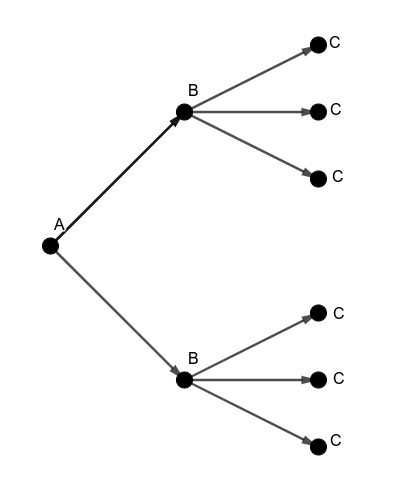
\includegraphics[scale = .3]{Images/tree_diagram_1.png}
\end{figure}

\begin{itemize}

\item Suppose we have three cities, $A$, $B$ and $C$. We need to go from $A$ to $C$ via $B$?  
\item If there are 2 ways we can go from $A$ to $B$ (call them \emph{path-$1$ and path-$2$}) and $3$ ways we can go from $B$ to $C$ (call them \alert{path-$3$, path-$4$ and path-$5$}), question is \emph{how many ways we go from $A$ to $C$ via $B$}? 
\item First note that the process has two parts, the first part we have \alert{$2$ possible ways} and in the second part we have \alert{$3$ possible ways}.
\item So the whole process can be performed in  $2 \times 3 = 6$ possible ways.   
\item For the multiplication problems, the tree diagram (figure below) could be useful to visualize.
\item We can list them using set (note that this is actually Cartesian Product of ....?)
\vspace*{-.4cm}

\begin{align*}
\{ (\text{Path-1, Path-3}), (\text{Path-1, Path-4}), (\text{Path-1, Path-5}), \\
(\text{Path-2, Path-3}), (\text{Path-2, Path-4}), (\text{Path-2, Path-5})\}
\end{align*}


\end{itemize}



\framebreak



\Thm{Example }(Multiplication Rule)
\begin{figure}[H]
\centering
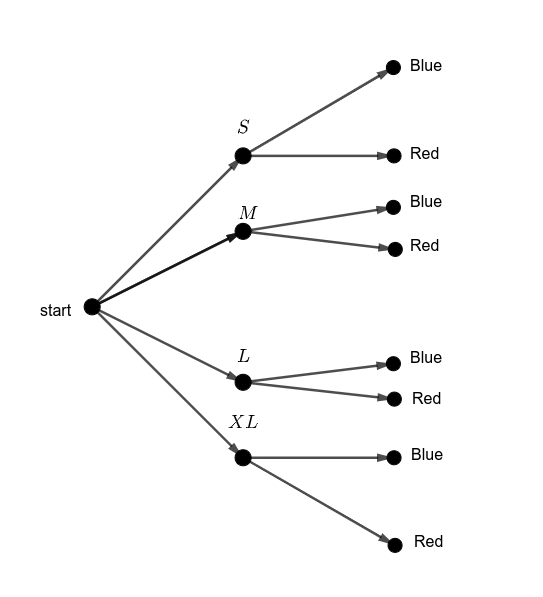
\includegraphics[scale = .25]{Images/tree_diagram_2.png}
\end{figure}

\begin{itemize}

\item Suppose a retail store sells \emph{windbreaker jackets} in \alert{sizes} small (S), medium (M), large (L), and extra large (XL). All are available in \alert{color} ``blue'' or ``red''. If a buyer wants to buy then \emph{how many options/choices are available for the buyer}? 


\medskip
\item Applying multiplication rule, we get in total there are $4 \times 2 = 8$ possible choices. Again we can write them using sets 


\medskip

\begin{dmath*} \{ (S, \text{Blue}), (S, \text{Red}), (M, \text{Blue}), \\
(M, \text{Red}), (L, \text{Blue}), (L, \text{Red}), \\
(XL, \text{Blue}), (XL, \text{Red}) \} \end{dmath*}

\end{itemize}




\framebreak

\item Now we can see the formal definition,

\begin{block}{Multiplication Rule}
If a procedure or a process consists of $k$ \alert{independent parts} (where $k \geq 2$) and the $i^{th}$ part can be performed in $n_i$ possible ways (where $i = 1, 2, \ldots, k$), then the entire process can be performed in $n_1 \times n_2 \times \ldots, \times  n_k$ possible ways.
\end{block}

\item Here $i^{th}$ part can be performed in $n_i$ possible ways means,

\begin{itemize}
  \item when $i = 1$, $1^{st}$ process can be performed with $n_1$ ways 
  \item when $i = 2$, $2^{nd}$ process can be performed with $n_2$ ways 
  \item $\vdots$
  \item when $i = k$, $k^{th}$ process can be performed with $n_k$ ways
\end{itemize}

\item \alert{independent parts} means one part is not dependent on the other. 


\framebreak

\item More examples,
\medskip

\item[] \Thm{Example }(Multiplication Rule)

\item \textbf{Question:} Suppose a coin is tossed $6$ times, how many possible outcomes are there? 

\medskip

\item \textbf{Ans:} Actually there will be $2 \times  2 \times 2 \times 2 \times 2 \times 2 = 2^6 = 36$ possible outcomes. Can you list all possible outcomes. For example one outcomes is $HTTHHH$ (can you think about the tree diagram here?). The Cartesian product of the set $\{H, T\}$ six times will give you all possible outcomes.  Can you draw the tree diagram (yes but this is cumbersome)?

\medskip
\item[]

\item[] \Thm{Example } (Multiplication Rule)


\item  \textbf{Question:} Suppose we have a $3$ digit combination lock where each digit can be from $0$ to $9$. How many possible combination locks we can set?

\medskip

\item \textbf{Answer:} There will be $10 \times 10 \times 10 = 10^3 = 1000$ possible combination locks. Can you draw the tree diagram (yes but this is cumbersome)?




\end{itemize}

\end{frame}


\subsection{b. Permutation}
\frame{\subsectionpage}


\begin{frame}[allowframebreaks]{Counting Methods - Permutation}

\begin{itemize}

\item So multiplication problem is quite simple, in the next problem we consider one special case of the problem where \emph{which comes first or second matters, or we say ordering matters}.

\item For the lock problem, first note we can think about the same problem in the following way, 

\item think about \emph{three empty boxes} and then we want to know \emph{how many possible ways we can fill the boxes?} 

\item For the first box we have $10$ possible options, for the second we also have $10$, and for the third we also have $10$. This gives the following picture 

\vspace*{.3cm}
\begin{figure}
\centering
\begin{tikzpicture}
\node[draw] at (0,0) {$10$}; 
\node[draw = none] at (.5,0) {$\times$}; 
\node[draw] at (1,0) {$10$};
\node[draw = none] at (1.5,0) {$\times$}; 
\node[draw] at (2,0) {$10$};
\end{tikzpicture}
\end{figure}
\vspace*{.3cm}

\item This means we have $10 \times 10 \times 10 = 1000$ possible options for locks. 

\item Note this is the same problem but we are thinking now with boxes, rather than tree diagram.

\framebreak



\item Now consider the same problem, but \emph{suppose we don't want any repetition, this means the same digit cannot appear more than once}. 

\item So we want all three digits to be different. For example we don't want to count $0,0,1$ or $1, 1, 1$ as possible count.

\item We can solve this problem using the box idea.

\item For the first place we have $10$ digits, for the second place we have $9$ digits, and for the third we have $8$ digits left, this means we have now

\vspace*{.3cm}
\begin{figure}
\centering
\begin{tikzpicture}
\node[draw] at (0,0) {$10$}; 
\node[draw = none] at (.5,0) {$\times$}; 
\node[draw] at (1,0) {$9$};
\node[draw = none] at (1.5,0) {$\times$}; 
\node[draw] at (2,0) {$8$};
\end{tikzpicture}
\end{figure}
\vspace*{.3cm}


\item So $10 \times 9 \times 8 = 720$ possible combinations.

\item So problem solved! 

\item Note we still solved this problem as a multiplication problem.

\framebreak

\item The last problem can be also understood \emph{as a ordering problem}, roughly this means a problem where \emph{ordering matters}.


\item In general for any ordering problem, we don't have to think about the combination lock, the idea is if we have $10$ digits $0, 1, 2, 3, 4, 5, 6, 7, 8, 9$, we ask \alert{how many ways we can order any $3$ digits}. 


\item And the answer is same $10 \times 9 \times 8 = 720$.

\item What if we order $10$ objects such that ordering matters, then the answer is $10 \times 9 \times 8 \times \ldots \times 1$

\item Which in short we write, $10!$ or we say \alert{$10$ factorial}.

\item Note for any non-negative integers $n$,

\begin{align*}
n! = n \times (n-1) \times (n-2) \times \ldots \times 1
\end{align*}


\item For example $5! = 5 \times 4 \times 3 \times 2 \times 1 = 120$, and $4! = 4 \times 3 \times 2 \times 1 = 24$, and $3! = 3 \times 2 \times 1 = 6$.

\item We define $0! = 1$,

\framebreak

\item So with this factorial idea we can now write the total number of orderings for three digits out of $10$, as



\begin{align*}
\frac{10!}{(10 - 3)!} = \frac{10!}{7!} = 10 \times 9 \times 8
\end{align*}

\item which is the famous \emph{formula for permutation} and we write this as $\Permute[10]{3}$, in general

\begin{block}{\Thm{Definition~} (Permutation)}
If we have $n$ objects and we want to order $k$ of them, then the total number of orderings is given by

\begin{align*}
\Permute[n]{k} = \frac{n!}{(n - k)!}
\end{align*}

\end{block}



 


\item \alert{Side Note}: \emph{Ques: What does it mean we say ``ordering matters?''}, Ans: this  means when we are counting we are treating $1,2,3$ and $2, 1, 3$ as a separate count, not as a same count.

\item Also note the word ``permutation'' in English just means ``rearrangement''. For example if we have three letters a,b,c then a another permutation (or ordering) is b,a,c. So when we ask total number of permutations, this is same asking total number of arrangements or total number of orderings.

\framebreak


\item So , in general if someone asks you ``if we have $n$ objects then how many ways we can order $k$ of them if we pick one at a time?'' the answer is 


\begin{align*}
\Permute[n]{k} = \frac{n!}{(n - k)!}
\end{align*}


\item Or you can think with the boxes, in this case you can think $n$ objects and $k$ empty boxes and we are trying to fill them one by one. 

\item And as you already understood, if we have $n$ objects and $n$ boxes, then $ \Permute[n]{n} = n!$ (here we used  $0! = 1$) This means $n!$ gives the total number of orderings when we want to order $n$ objects and we have $n$ empty boxes.

\item Let's do some examples.






\framebreak



\item Ques: If we have $5$ letters $a, b, c, d, e$, then

\begin{itemize}
\item a) How many ways we can order them?
\item b) How many ways we can order $3$ of them (taking one at a time)?
\end{itemize} 

\item The answer of a) is $5! = 5 \times 4 \times 3 \times 2 \times 1 = 120$. 


\item To answer b), we can follow one of the two approaches\blfootnote{There is a nice website which can show all possible permutations, check this out - \url{https://www.dcode.fr/partial-k-permutations}}

\medskip

\begin{itemize}
\item \textbf{Empty box approach (perhaps this is more intuitive):} We have $3$ empty boxes, so for the first box we have $5$ options, for the second box we have $4$ and for the third we have $3$. So in total we have $5 \times 4 \times 3 = 60$. So there are $60$ possible ways we can order them 

\medskip

\item \textbf{Directly applying the formula:} Since this is a direct ordering problem we can apply the permutation formula, $\Permute[5]{3} = \frac{5!}{(5 - 3)!} = 60$.
\end{itemize}


\item Here are all $60$ permutations if we pick $3$ letters out of $5$.


\begin{align*}
\begin{array}{llllll}
a,b,c &
b,a,c &
c,a,b &
a,c,b &
b,c,a &
c,b,a \\
a,b,d &
b,a,d &
d,a,b &
a,d,b &
b,d,a &
d,b,a \\
a,b,e &
b,a,e &
e,a,b &
a,e,b &
b,e,a &
e,b,a \\
a,c,d &
c,a,d &
d,a,c &
a,d,c &
c,d,a &
d,c,a \\
a,c,e &
c,a,e &
e,a,c &
a,e,c &
c,e,a &
e,c,a \\
a,d,e &
d,a,e &
e,a,d &
a,e,d &
d,e,a &
e,d,a \\
b,c,d &
c,b,d &
d,b,c &
b,d,c &
c,d,b &
d,c,b \\
b,c,e &
c,b,e &
e,b,c &
b,e,c &
c,e,b &
e,c,b \\
b,d,e &
d,b,e &
e,b,d &
b,e,d &
d,e,b &
e,d,b \\
c,d,e &
d,c,e &
e,c,d &
c,e,d &
d,e,c &
e,d,c &
\end{array}
\end{align*}

\item It's important that you understand the phrase \emph{``ordering matters''} in the permutation problem, 

\item In our example this means when we pick three letters we take all possible permutations when we do the counting, for example, take the first row where we have different permutations of the letter $a, b, c$. In total there are $3 \times 2 = 6$ permutations,.... ordering matters means when we count, we count all $6$ of them. 

\item Similarly in every row we have $6$ permutations of three letters and when we count we count all of them.

\item \textbf{Question:} \emph{What if we treat them as a single count?}

\end{itemize}
\end{frame}

\subsection{c. Combination}
\frame{\subsectionpage}


\begin{frame}[allowframebreaks]{Counting Methods - Combination}


\begin{itemize}
\item The answer to last question lies in the idea of \emph{combination problem}. In the combination problem we use the idea of \emph{``selection''}, rather than ordering, and we count all permutations of the same objects as one count.

\item For example, in the last letter problem, if we ask \emph{``how many ways we can \alert{select} $3$ letters out of $5$ letters'', the answer is $10$} (notice the word ``select'' here)

\item Here ``select'' means, we are just selecting and we don't care about orders now.

\item Now how did we get $10$? Just count one for each row where we show all possible permutations. Since there are $10$ rows we have $10$ possible combinations. We can reach this by dividing the excess count, here is the formal definition,


\framebreak



\begin{block}{\Thm{Definition } (Combinations)}
If we have a set of $n$ elements. Each \emph{subset} of size $k$ chosen from this set is called a \alert{combination of $n$ elements taken $k$ at a time}. We denote the number of \alert{distinct} such combinations by the symbol $\Combine[n]{k}$. And we can count this number by

$$
\Combine[n]{k}=\frac{\Permute[n]{k}}{k!} = \frac{n !}{k !(n-k) !}
$$

\end{block}

\framebreak



\item There is another way to understand the formula, the idea is let's think in this case the number of permutations being constructed in two steps or two parts. 

\item \emph{Part 1:} How many ways we can select $k$ elements from $n$, this is $\Combine[n]{k}$ (this is the selection part)

\item \emph{Part 2} How many ways those $k$ elements can be arranged / ordered within themselves. This is $k!$

\item Now if we apply the multiplication rule and we get the total number of orderings,


\begin{align*}
\Permute[n]{k} = \Combine[n]{k} \times k!
\end{align*}



\item and from here we get our formula

\begin{align*}
\Combine[n]{k}=\frac{\Permute[n]{k}}{k!}
\end{align*}

\framebreak

\item Also note we can say - the number of distinct subsets of size $k$ that can be chosen from a set of size $n$ is $\Combine[n]{k}$.

\item Or if someone asks you \alert{``how many ways you can select $k$ objects from $n$?''}, then the answer is  $\Combine[n]{k} = \frac{\Permute[n]{k}}{k!} = \frac{n !}{k !(n-k) !}$


\item There is another notation for the combination and that is $\left(\begin{array}{l}
n \\
k
\end{array}\right)$ 

\item So  $\left(\begin{array}{l}
n \\
k
\end{array}\right)$  is same as $\Combine[n]{k}$, it means \alert{``how many distinct ways we can select $k$ objects from $n$?''}



\end{itemize}


\end{frame}

%------------------------------------------------------------------------------------------------
%------------------------------------------------------------------------------------------------
\begin{frame}{Counting Methods}
\framesubtitle{Binomial theorem}
There is a very useful application of $\Combine[n]{k}$, we this call \emph{Binomial Theorem}, here is the theorem.
\begin{block}{\Thm{Theorem } (Binomial Theorem.)}
For all numbers $x$ and $y$ and each positive integer $n$,

$$
(x+y)^{n}=\sum_{k=0}^{n}\left(\begin{array}{l}
n \\
k
\end{array}\right) x^{k} y^{n-k} .
$$


where $\left(\begin{array}{l}
n \\
k
\end{array}\right)$ is same as $\Combine[n]{k}$, so this is possible number of combinations of $k$ objects out of $n$. In this case this is also known as \emph{Binomial co-efficient}


\end{block}




\end{frame}




% \bibliographystyle{plainnat}
% \bibliography{../common/refs}

\end{document}
